
\documentclass[runningheads,a4paper]{llncs}

\usepackage{array}
\usepackage{epsfig}
\usepackage[all]{xy}
\usepackage{enumerate}
\usepackage{graphicx}
\usepackage{tikz}
\usepackage{xspace}
\usepackage{float}
\usepackage{comment}

%%%% Packages needed by Matteo
\usepackage[all]{xy}
\usepackage{stmaryrd}
\usepackage{amssymb}
\usepackage{amsmath}
\usepackage{verbatim}


%%%% End of Packages needed by Matteo

\newcommand{\fun}[3]{\ensuremath{#1\colon #2 \to #3}}
\newcommand{\parfun}[3]{\ensuremath{#1\colon #2 \rightharpoonup #3}}

%%%%%%%%%%%%%%%%%%%%%%%%%%%%%%%%
%
%
% The record
%
%
%%%%%%%%%%%%%%%%%%%%%%%%%%%%%%%%

\newcommand{\therecord}{{$84$}\ }
\newcommand{\theoctagons}{{$126912$}\ }
\newcommand{\theinstances}{{$42889$}\ }

%%%%%%%%%%%%%%%%%%%%%%%%%%%%%%%%
%
%
% The biblatex requirements 
%
%
%%%%%%%%%%%%%%%%%%%%%%%%%%%%%%%%

\usepackage[backend=bibtex]{biblatex}
\bibliography{games.bib}

%%%%%%%%%%%%%%%%%%%%%%%%%%%%%%%
%
%
% Stuff needed for pictures
%
%
%%%%%%%%%%%%%%%%%%%%%%%%%%%%%%%%

%\usepackage[usenames,dvipsnames]{xcolor}
\usepackage{tikz}
\usepackage{xifthen}
\usepackage{intcalc}
\usetikzlibrary{calc}
\usetikzlibrary{arrows}
\usepackage{pgfplots}
\usepackage{wrapfig}
\usepackage[font={scriptsize,it}]{caption}
\usepackage{cutwin}
%\usepackage{picins}


%%%%%%%%%%%%%%%%%%%%%%%%%%%%%%%%
%
%
% Added for the sake of internal 
% references
%
%
%%%%%%%%%%%%%%%%%%%%%%%%%%%%%%%%

\usepackage{enumitem, hyperref}
\makeatletter
\def\namedlabel#1#2{\begingroup
    #2%
    \def\@currentlabel{#2}%
    \phantomsection\label{#1}\endgroup
}

%%%%%%%%%%%%%%%%%%%%%%%%%%%%%%%%
%
%
% Added to have a sane enumeration 
% of conditions in Lemma 4 (o1)-(o8)
%
%
%%%%%%%%%%%%%%%%%%%%%%%%%%%%%%%%

\usepackage{mathtools} 

%%%%%%%%%%%%%%%%%%%%%%%%%%%%%%%%
%
%
% Commands needed by Andrzej
%
%
%%%%%%%%%%%%%%%%%%%%%%%%%%%%%%%%


%\usepackage[english]{babel}
\usepackage[utf8]{inputenc}
\usepackage{graphicx}
%\usepackage{amsthm}
\usepackage{amsmath}
\usepackage[colorinlistoftodos]{todonotes}


\numberwithin{equation}{section}

%\newtheorem{theorem}{Theorem}[section]
%\newtheorem{lemma}[theorem]{Lemma}
%\newtheorem{corollary}[theorem]{Corollary}
%\newtheorem{proposition}[theorem]{Proposition}
%\newtheorem{conjecture}[theorem]{Conjecture}
%\newtheorem*{theorem*}{Theorem}

%\theoremstyle{definition}
%\newtheorem*{definition}{Definition}
%\newtheorem{example}[theorem]{Example}
\newtheorem{xca}[theorem]{Exercise}

%\theoremstyle{remark}
%\newtheorem{remark}[theorem]{Remark}
%\newtheorem{question}[theorem]{Question}
%\newtheorem*{remark*}{Remark}
\newtheorem*{convention*}{Convention}
\newtheorem*{notation*}{Notation}

\DeclareMathOperator{\hull}{hull}
\DeclareMathOperator{\external}{ex}
\DeclareMathOperator{\modifier}{modifier}
\DeclareMathOperator{\internal}{int}
\DeclareMathOperator{\gap}{gap}
\DeclareMathOperator{\param}{param}
\DeclareMathOperator{\bd}{\partial}
\DeclareMathOperator{\pot}{potential}
\DeclareMathOperator{\dt}{dot}
\DeclareMathOperator{\move}{mv}
\DeclareMathOperator{\obj}{obj}
\DeclareMathOperator{\oct}{octagon}


\renewcommand{\comment}[1]{}


\newcommand {\nat}{\mathbb{N}}
\newcommand {\scc}{\mathsf{scc}}
\newcommand {\ord}{\mathsf{ORD}}
\newcommand {\un}{\mathsf{un}}
\newcommand {\head}{\mathsf{head}}
\newcommand {\tail}{\mathsf{tail}}
\newcommand {\ad}{\mathsf{ad}}
\newcommand {\sub}{\mathsf{sub}}
\newcommand {\dom}{\mathsf{dom}}
\newcommand {\rank}{\mathsf{rank}\xspace}
\newcommand {\red}{\mathsf{red}}
\newcommand {\LGA}{\mathsf{LGA}}
\newcommand {\WAA}{\mathsf{WAA}}
\newcommand {\SAA}{\mathsf{SAA}}
\newcommand {\mybox}{\textrm{{\scriptsize $\,\Box\,$}}}
\newcommand {\R}{${\mathcal R}$}
\newcommand {\RR}{{\mathcal R}}
\newcommand {\C}{${\mathcal C}$}
\newcommand {\BC}{\mathsf{BC}}


\newcommand{\dotcup}{\ensuremath{\mathaccent\cdot\cup}}


% Letters and numbers

\newcommand{\mathromnum}[1]{\ensuremath{\mathrm{#1}}\xspace}

\newcommand{\rI}{\mathromnum{I}}
\newcommand{\rII}{\mathromnum{II}}
\newcommand{\rIII}{\mathromnum{III}}
\newcommand{\rIV}{\mathromnum{IV}}
\newcommand{\rV}{\mathromnum{V}}

\newcommand{\mathcalsym}[1]{\ensuremath{\mathcal{#1}}\xspace}

\newcommand{\Cross}{\texttt{Cross}}
\newcommand{\Aa}{\mathcalsym{A}}
\newcommand{\Bb}{\mathcalsym{B}}
\newcommand{\Cc}{\mathcalsym{C}}
\newcommand{\Dd}{\mathcalsym{D}}
\newcommand{\Ee}{\mathcalsym{E}}
\newcommand{\Ff}{\mathcalsym{F}}
\newcommand{\Gg}{\mathcalsym{G}}
\newcommand{\Hh}{\mathcalsym{H}}
\newcommand{\Ii}{\mathcalsym{I}}
\newcommand{\Jj}{\mathcalsym{J}}
\newcommand{\Kk}{\mathcalsym{K}}
\newcommand{\Ll}{\mathcalsym{L}}
\newcommand{\Mm}{\mathcalsym{M}}
\newcommand{\Nn}{\mathcalsym{N}}
\newcommand{\Oo}{\mathcalsym{O}}
\newcommand{\Pl}{\mathcalsym{P}}
\newcommand{\Ql}{\mathcalsym{Q}}
\newcommand{\Rr}{\mathcalsym{R}}
\newcommand{\Ss}{\mathcalsym{S}}
\newcommand{\Tt}{\mathcalsym{T}}
\newcommand{\Uu}{\mathcalsym{U}}
\newcommand{\Vv}{\mathcalsym{V}}
\newcommand{\Ww}{\mathcalsym{W}}
\newcommand{\Xx}{\mathcalsym{X}}
\newcommand{\Yy}{\mathcalsym{Y}}
\newcommand{\Zz}{\mathcalsym{Z}}
\newcommand{\W}{\mathrm{W}}
\newcommand{\coR}{\mbox{co-}\Rr}

%-------------------------------

\newcommand{\trees}{\mathrm{Tr}\xspace}
\newcommand{\runs}{\mathrm{Runs}\xspace}
\newcommand{\otrees}{\mathrm{Tr}(\omega)\xspace}
\newcommand{\WF}{\mathrm{WF}\xspace}


\newcommand{\boldclass}[3]{\ensuremath{\mathbf{#1}^{#2}_{#3}}}
\newcommand{\lightclass}[3]{\ensuremath{{#1}^{#2}_{#3}}}

\newcommand{\borel}{\ensuremath{\mathcal B}\xspace}

\newcommand{\bsigma}[1]{\boldclass{\Sigma}{0}{#1}}
\newcommand{\bpi}[1]{\boldclass{\Pi}{0}{#1}}
\newcommand{\bdelta}[1]{\boldclass{\Delta}{0}{#1}}

\newcommand{\asigma}[1]{\boldclass{\Sigma}{1}{#1}}
\newcommand{\api}[1]{\boldclass{\Pi}{1}{#1}}
\newcommand{\adelta}[1]{\boldclass{\Delta}{1}{#1}}

\newcommand{\esigma}[2]{\lightclass{\Sigma}{#1}{#2}}
\newcommand{\epi}[2]{\lightclass{\Pi}{1}{#1}}
\newcommand{\edelta}[2]{\lightclass{\Delta}{#1}{#2}}


\newcommand{\bc}[1]{\mathcal{BC}({#1})}

\newcommand{\textscsym}[1]{{\sc #1}}

\newcommand{\eqdef}{\stackrel{\mathrm{def}}=}

\newcommand{\N}{\nat}

%\newcommand{\dL}{\mathrm{L}}
%\newcommand{\dR}{\mathrm{R}}

\newcommand{\rmin}{i}
\newcommand{\rmax}{k}

\newcommand{\G}{\mathcal{G}}

\newcommand{\Plab}{{\mathrm{label}}}
\newcommand{\guarantee}{{\mathrm{promise}}}

\newcommand{\Pgar}{X}

\newcommand{\eve}{\ensuremath{\exists}\xspace}
\newcommand{\adam}{\ensuremath{\forall}\xspace}

\newcommand{\ZFC}{{\sc ZFC}}
\newcommand{\LTL}{{\sc LTL}}
\newcommand{\CTL}{{\sc CTL}}
\newcommand{\PCTL}{{\sc PCTL}}
\newcommand{\CTLstar}{{\sc LTL$^\ast$}}
\newcommand{\ZFCMA}{{\sc ZFC+MA$_{\aleph_{1}}$}}
\newcommand{\MA}{{\sc MA$_{\aleph_{1}}$}}
\newcommand{\ZFCVL}{{\sc ZFC+V=L}}
\newcommand{\VL}{{\sc V=L}}
\newcommand{\AD}{{\sc AD}}
\newcommand{\CH}{{\sc CH}}

\newcommand{\powerset}{{\mathcal P}}
\newcommand{\la}{{\langle}}
\newcommand{\ra}{{\rangle}}

\newcommand{\hargame}{{H\Gg}}

\newcommand{\restr}{\!\upharpoonright}

\newcommand{\ignore}[1]{}
\newcommand{\Souslin}{\mathcal A}


\newenvironment{proofof}[1]
	{\vspace{1ex}\noindent{\emph{Proof of #1}}\hspace{0.5em}}
    {\hfill\qed\vspace{1ex}}
    
%%%%%%%%%%%%%%%%%%%%%%%%%%%%%%%%%%%%
%
%
% acknowledgments on the front page
%
%
%%%%%%%%%%%%%%%%%%%%%%%%%%%%%%%%%%%%    

\newcommand*\samethanks[1][\value{footnote}]{\footnotemark[#1]}


\lstdefinestyle{myCustomPythonStyle}{
  language=Python,
  numbers=left,
  stepnumber=1,
  numbersep=10pt,
  tabsize=4,
  showspaces=false,
  showstringspaces=false,
  basicstyle=\ttfamily\small
}





\author{Henryk Michalewski %\thanks{Deep thanks to all sponsors.} 
\and Andrzej Nagórko\and Jakub Pawlewicz}
%
\authorrunning{H.~Michalewski, A.~Nagórko, J.~Pawlewicz} %Lecture Notes in Computer Science: Authors' Instructions}
% (feature abused for this document to repeat the title also on left hand pages)

% the affiliations are given next; don't give your e-mail address
% unless you accept that it will be published
\institute{University of Warsaw\\
Faculty of Mathematics, Informatics, and Mechanics\\
\email{\{H.Michalewski,A.Nagorko,J.Pawlewicz\}@mimuw.edu.pl}}

%
% NB: a more complex sample for affiliations and the mapping to the
% corresponding authors can be found in the file "llncs.dem"
% (search for the string "\mainmatter" where a contribution starts).
% "llncs.dem" accompanies the document class "llncs.cls".
%

%\toctitle{Lecture Notes in Computer Science}
%\tocauthor{Authors' Instructions}

\begin{document}

\title{\therecord - a new upper bound for Morpion Solitaire}
\maketitle

\begin{abstract}
%We express properties of a Morpion~5T position graph by a linear program.
In \cite{demaine} an upper bound of 705  was proved on the number of moves in the 5T variant of the Morpion Solitaire game. We show a new upper bound of \therecord moves. This is achieved in the following way: we encode Morpion 5T rules as a linear program and solve \theoctagons instances of this program on 
%restrict the infinite grid on which the Morpion~5T game is played to one of 
 special octagonal boards. % and solve linear programs encoding Morpion 5T positions on these boards.
In order to show correctness of this method we analyze rules of the game and use a concept of a potential of a given position. By solving continuous-valued relaxations of linear programs on these boards, we obtain an upper bound of $586$ moves.
Further analysis of original, not relaxed, mixed-integer programs leads to an improvement of this bound to \therecord moves. However, this is achieved at a significantly higher computational cost. 
\end{abstract}

\section{Introduction}
The Morpion Solitaire is a paper-and-pencil single-player game played on a square grid with 
  the initial configuration of 36 dots depicted in Figure~\ref{fig:initial}. 
In each move the player puts a dot on an unused grid position and draws a line that 
  consists of four consecutive segments passing through the dot. 
The line must be horizontal, vertical or diagonal. 
The goal is to find the longest possible sequence of moves.
There are two main variants of the game: 5T and 5D. 
They have different restrictions on how the moves may be placed.
In the 5T variant of the game, no segment may be drawn twice, i.e. the moves have to be segment-disjoint. 
In the 5D variant of the game, any two moves in the same direction have to be dot-disjoint.
The difference is demonstrated in Figure~\ref{fig:initial}.\todo{Complete the figure}
% The 5D variant is more restrictive. In Morpion 5D there has to be a gap between moves placed on a same line.

  \begin{figure}
    \centering
      \includegraphics[width=0.49\textwidth]{figures/empty.pdf}
      \includegraphics[width=0.49\textwidth]{figures/empty.pdf}
      \caption{\label{fig:initial}
	The initial position of Morpion Solitaire is depicted on the right. On the left there is a position which is up to $4$--th move legal 
both in Morpion 5D and Morpion 5T variants, but the $5$--th move is legal only in Morpion 5T. 
      }
\end{figure}

The problem is notoriously hard for computers. 
For $34$ years the longest known sequence in the Morpion 5T game
  was one of 170 moves discovered by C.-H. Bruneau in $1976$. 
Despite considerable computational effort, until $2010$ the computer generated
  sequences were much shorter. 
In $2010$ Rosin \cite{rosin} obtained the current world records of $178$ moves in Morpion 5T 
  and of $82$ moves in Morpion 5D using a specialized Monte Carlo algorithm. This work  was
   recognized as a best paper of the IJCAI conference in 2011. The webpage~\cite{boyer} maintained by Christian Boyer, contains an extensive and up-to-date information about records in all Morpion Solitaire variants.

\subsection{Morpion Solitaire and linear programming}
The rules of Morpion Solitaire do not limit the size of the grid on which the game is played, hence a priori
  it is not clear if the sequences have to be bounded.
%A popular magazine \emph{Science \& Vie} published in $1970$'s different bounds submitted by its readers for the maximal length of a sequence in Morpion 5T  (the bounds ranged from $540$ to $20736$), but without detailed and/or valid proofs.
%The first rigorously proved bound of $705$ in Morpion 5T was published in $2006$ \cite[Demaine et al.]{demaine}.
%The best known bound of $485$ in Morpion 5T was proved in~\cite{ijcai}.
%In this paper we prove an upper bound of $84$ on the length of Morpion 5D sequence, 
%improving upon a bound of $121$ found earlier by \cite[Kawamura et al.]{japonczycy}.
%\begin{comment}
%Proofs of upper bounds discussed above exploit geometric and combinatorial properties of graphs that are obtained as Morpion Solitaire positions. 
%To set the mood we'll discuss the bound of $705$ moves for Morpion 5T as it was proved in~\cite{demaine}.
%A position of a Morpion Solitaire gameplay (Figure~\ref{fig:small}) has a graph structure.
%Its vertices are placed in the $\mathbb{Z}^2$ grid.
%Let $n$ denote the number of vertices, 
%  corresponding both to the dots placed by moves and to the dots from the starting cross.
%The edges correspond to the segments placed on the grid by moves.
%Every move adds a single vertex and four edges to the graph.
%Therefore a Morpion position graph has the following two properties: 1) its edges have unit length in $\ell_\infty$ metric; 2) $4n - e = 4 \cdot 36 = 144$. \todo{I do not like the idea of putting here $n%%$, $e$, $l_\infty$ and basically I am afraid that someone less patient may stop reading here without getting to the main result - maybe we can make a picture instead of this?}
%In~\cite{brass} P. Brass proved that if a planar graph $G$ has $n$ vertices, 
%  then the maximum number of edges in $G$ that have unit length in $\ell_\infty$ metric is equal to
%  $
%    s(n) = \lfloor 4n - \sqrt{28n - 12} \rfloor.
%  $
%Hence
%$
%  4n - 144 = e \leq s(n) = \lfloor 4n - \sqrt{28n - 12} \rfloor.
%$
%The maximal $n$ that satisfies this inequality is $n = 741$. 
%Considering the initial $36$ dots this gives an upper bound of $705$ on the number of moves 
%  in Morpion Solitaire~\cite{demaine}.
%  
%Observe that the Morpion position graph has additional geometrical property.
%The set of its edges may be covered by a set of segment-disjoint \emph{moves} consisting of four consecutive, parallel, distinct unit length segments. 
%We call such graphs \emph{unmarked unordered Morpion graphs} (see Section~\ref{sec:linear} for formal definitions).
% In~\cite{ijcai} we used linear programming to show a bound of $485$ on the number of vertices in such a graph, under additional constraints about the size of its bounding box  that follow from rules of %%Morpion 5T and from a variant of an isoperimetric inequality. %\todo{The same stuff as one paragraph below}
%\end{comment}
 %\todo{Insert why the game is epxressible via a linear program}
However, as a single player game, Morpion Solitaire can be  encoded in a natural way as a linear optimization problem with the optimization target being the length of the sequence. On its own the encoding is not very helpful, because the problem is too large to be practically solvable. Nevertheless, this inspires a natural approach towards construction of upper bounds. Instead of solving the Morpion Solitaire, we solve
a more general game such that
\begin{itemize}
\item every gameplay of ordinary  Morpion Solitaire is a gameplay of the generalization,
\item the generalization is practically solvable and
\item an upper bound proved for this more general game is still interesting for the Morpion Solitaire. 
\end{itemize}
We do not expect that the more general game will be playable by humans. Here is a summary of results we managed to obtain using this approach:
\begin{itemize}
\item the %first rigorously proved 
bound of $705$ in Morpion 5T was proved in $2006$ in \cite[Demaine et al.]{demaine} using a careful geometric analysis of moves in Morpion 5T and a potential argument. The current best bound of $485$ in Morpion 5T was obtained in~\cite{ijcai} using an appropriate generalization of Morpion 5T. In particular in \cite{ijcai} it was shown that the bound of $586$ can be obtained via the relaxation of the linear program encoding the rules of  Morpion 5T;
\item a geometric analysis of Morpion 5D led in \cite[Kawamura et al.]{japonczycy} to an upper bound of $121$ which improved on an earlier bound of $144$ found in \cite{demaine} using the potential method; using a generalization of Morpion 5D, in this paper we prove an upper bound of $84$ on the length of Morpion 5D sequences;
%, improving upon a bound of $121$ found earlier by  using a geometrical analysis of moves in Morpion 5D. 
% will significantly improve on the above geometric bounds \cite[Kawamura et al.]{japonczycy};  
%A certain generlization of Morpion Solitaire 5T we analyzed in \cite{ijcai}, however this method 
the method used in  \cite{ijcai} does not seem very helpful in Morpion 5D --- later in this paper we discuss differences between these two generalizations. 
\end{itemize}

%\begin{comment}  
%In the present paper we shall use additional combinatorial property of Morpion graphs:
%one can find an assignment such that to each move is assigned one of its dots and the assignment is one-to-one (see Section \ref{sec:linear} for a precise definition).
%We call such graphs \emph{unordered Morpion graphs}. % (Figure~\ref{fig:85}).
%Every Morpion 5D gameplay generates such assignment but there are assignments 
%which are not generated by any gameplay (see example of such situation in Figure\ref{fig:85})
%\end{comment} 

%\todo{The following paragraph should be written in a different way --- emphasize Theorem, maybe Lemmas, the table} 
\subsection{Organization of the paper}
In Section \ref{sec:geometry} we formulate the main results:
\begin{itemize}
\item in Theorem \ref{thm:boxes} we show that every Morpion 5D gameplay must be contained in a relatively small rectangular box around the starting cross in Figure \ref{fig:initial}; this already proves the bound of $85$ in Morpion 5D,
\item in Corollary \ref{cor:84} we improve this bound to 84 through an analysis of $4$ special cases.
\end{itemize}
The proof of these results is divded between next three sections. In Section \ref{sec:linear} we define a useful generalization of Morpion 5D 
and encode it as a linear program. In Section \ref{sec:gemmating} we generate a list of rectangular boards (``boxes'') such that any position of morpion 5D is contained in one of the boxes --- this is achieved using an auxilliary linear program. In Section \ref{sec:upper} we solve 
the generalization of Morpion 5D on all boards found in Section \ref{sec:gemmating} and conclude the proof of Theorem \ref{thm:boxes} along with Corollary \ref{cor:84}. Moreover, we apply the same approach to symmetric variants of Morpion 5T and Morpion 5D and solve completely these
two games.

%We prove that the
%  size of graphs with these combinatorial and geometrical properties does not exceed $85$.
%We will also use additional constraint about a size of the bounding box of the graph that follows from
%  calculations combined with the rules of the game.
%We then use additional argument to show that the graphs of size $85$ do not correspond to Morpion positions.

%In~\cite{ijcai} we used isoperimetric inequality combined with mixed integer programming to obtain an upper bound of $485$ for Morpion 5T. 
%The method employed in~\cite{ijcai} does not give useful upper bound for the 5D variant.
%In the present paper we use a new technique of gemmating to limit the size of a bounding box of a Morpion 5D graph combined with a new reduction of Morpion Solitaire to a mixed integer programming to obtain a bound of $84$ for Morpion 5D. \todo{List precisely results which are important for this paper}


% !TEX root = main.tex

\section{Linear Relaxation}
\label{linear}

% Lattice graph, move.

A \emph{lattice point} on a plane is a point with integer coordinates. A \emph{lattice graph} is a graph with vertices in lattice points and edges consisting of pairs $(p,q)$, where $p$ and $q$ are two different neighboring points, that is $p\neq q$ and $p=(n,m)$ and $q=(n\pm i,m\pm j)$ for some $i,j=0,1$. %Notice, that edges are congruent to segments from the point $(0,0)$ to one of the points $(0, 1), (0, 1), (1, 1), (1, 0)$.
We call such edges the \emph{lattice edges}.

% Morpion graph.

A \emph{move} in a lattice graph $G = (V, E)$ is a set of four consecutive parallel lattice edges. 
%The four edges must be horizontal, vertical or diagonal. 
We let $\mathcal{M}(G)$ to be the set of all moves in a graph $G$.
We start with the following observation, which simply rephrases the rules of Morpion 5T++ formulated in the Introduction. 

\begin{lemma}%\todo{Optional: change this into a definition and just remark, that incidentally these are Morpion 5++ positions. This would save us a bit of work related to explanation of Morption 5++ tules.}
\label{lem:char5pluplus}
A graph $G = (V, E)$ is a Morpion 5T++ position graph if and only if it satisfies the following conditions
  \begin{enumerate}
  \item[\namedlabel{m1}{(M1)}] $G$ is a lattice graph,
  \item[\namedlabel{m2}{(M2)}] $4 \cdot \# V - \# E = 144$,
  \item[\namedlabel{m3}{(M3)}] The set $E$ of edges of $G$ can be decomposed into a collection of disjoint moves.
  \end{enumerate}
\end{lemma}
%\begin{proof}
%  basically induction on the number of moves (but we have a stash of unused dots)
%\end{proof}

% Linear constraints on 5++ position.

Let $B = (V_B, E_B)$ be a fixed lattice graph that we shall call \emph{the board}. 
In applications, it will be a sufficiently large octagonal lattice graph with a full set of edges.
Below we define linear constraints that describe all subgraphs of $B$ that satisfy conditions \ref{m1}--- \ref{m3} of Lemma~\ref{lem:char5pluplus}.

We define the following set of structural {\em binary} variables, that is variables assuming values $0,1$:
\[
  \tag{LP1}
  \{ \dt_v \colon v \in V_B \} \cup \{ \move_m \colon m \in \mathcal{M}(B) \}.
  \label{lp1}
\]

\noindent
For each $e \in E_B$ and $v \in e$ we declare the following constraints:
\begin{equation}
  \tag{LP2}  \sum_{ m \in \mathcal{M}(B), e \in m } \move_m \leq \dt_v.
  \label{lp2}
\end{equation}

\begin{equation}
  \tag{LP3} \sum_{v \in V_B} \dt_v = 36 + \sum_{m \in \mathcal{M}(B)} \move_m. 
  \label{lp3}
\end{equation}

The following two lemmas describe correspondence between binary-valued solutions of a mixed integer programming problem (\ref{lp1}) - (\ref{lp3}) and subgraphs of $B$ that are Morpion 5T++ positions.

\begin{lemma} Let $G=(V_G,E_G)$ be a subgraph of $B$ and a Morpion 5T++ position obtained by a sequence $\mathcal{M}$ of moves. If
\[
  \dt_v = \left\{ 
    \begin{array}{ll}
      0 & \text{ if } v \not\in V_G \\
      1 & \text{ if } v \in V_G
    \end{array}
  \right.
    \text{ and }
  \move_m = \left\{ 
    \begin{array}{ll}
      0 & \text{ if } v \not\in \mathcal{M} \\
      1 & \text{ if } v \in \mathcal{M}
    \end{array}
  \right.,
\]
then conditions (\ref{lp1}), (\ref{lp2}) and (\ref{lp3}) hold. 
\end{lemma}

\begin{proof}
If $\dt_v=0$, then there is no move passing through $v$, hence the left hand side of (\ref{lp2}) is equal to $0$. If $\dt_v=1$, then  condition (\ref{lp2}) means that every segment $e$ played in the game can appear in exactly one move.  Condition (\ref{lp3}) means that the number of dots placed is higher by 36 than the number of moves made.
\end{proof}

\begin{lemma} Assume that a set of variables defined by condition (\ref{lp1}) satisfies conditions (\ref{lp2}) and (\ref{lp3}).
Let $G = (V_G, E_G)$ be a graph with a set of vertices
\[
  V_G = \{ v \in V_B \colon \dt_v = 1 \}
\]
and a set of edges
\[
  E_G = \{ e \in E_B \colon \exists_{m \in \mathcal{M}(B)}\ e \in m, \move_m = 1 \}.
\]
Then $G$ is a Morpion 5T++ position and a subgraph of $G$. 
\end{lemma}
\begin{proof}
%Assume that we have a feasible binary-valued solution of the linear programming problem, that is
% we have $\dt_v, \move_m \in \{ 0, 1 \}$ such that \ref{lp1}--\ref{lp3}  holds.
We will show that $G$ satisfies conditions \ref{m1} --- \ref{m3} of Lemma~\ref{lem:char5pluplus}.

By the definition of $E_G$, if $e \in E_G$ then there exists $m \in \mathcal{M}(B)$ such that $\move_m = 1$.
By (\ref{lp2}), if $\move_m = 1$, then $\dt_v = 1$ for each $v \in V_B$ such that $v \in e \in m$. It means that graph $G$ contains vertices of its edges, therefore it is a well defined subgraph of $B$, hence it is a lattice graph and it satisfies \ref{m1}. 

From (\ref{lp2}) follows, that the moves $\move_m$ must be disjoint in the sense, that they cannot contain the same edge twice. This implies condition \ref{m3} of Lemma \ref{lem:char5pluplus}. From disjointness and condition (\ref{lp3}) follows condition \ref{m2} of Lemma \ref{lem:char5pluplus}.
\end{proof}

% LPP

We consider a linear relaxation of the MIP problem (\ref{lp1})---(\ref{lp3}). We let structural variables to be real-valued, subject to bounds
\begin{equation}
  \tag{LP4} 0 \leq \dt_v, \move_m \leq 1.
  \label{lp4}
\end{equation}
\noindent
In the relaxation we maximize the objective function 
\begin{equation}
  \tag{LP0} \sum_{m \in \mathcal{M}(B)}  \move_m  % \rightarrow max.
  \label{lp0}
\end{equation}%\todo{Shouln't it be formulated before the Lemma? Otherwise what is optimized there?}
Clearly, an optimal solution to the linear programming problem (LP0) - (LP4) gives an upper bound for the length of a Morpion 5T++ game on a board $B$.

\subsection{The problem of the infinite grid}
\label{inf_grid}

Observe that any lattice graph that consists of $9$ vertex-disjoint moves has $45$ vertices and $36$ edges and satisfies conditions \ref{m1} --- \ref{m3} of Lemma~\ref{lem:char5pluplus}, hence it is a Morpion 5T++ position graph and consequently Morpion 5T++ positions can have arbitrarily large diameter in the plane ${\mathbb R}^2$.

The following table summarizes solutions of the linear relaxation of Morpion 5T++ on square $n \times n$ boards (where $n$ is the number of edges on the side).% with $n = 10, \ldots, 100$.
%\todo{Tell about the reference machine.}
\begin{figure}[H]

\bgroup
\def\arraystretch{1.5}
\setlength\tabcolsep{1mm}
\begin{tabular}{|c|c|c|c|c|c|c|c|c|c|}
\hline
10 & 20 & 30 & 40 & 50 & 60 & 70 & 80 & 90 & 100 \\
\hline
64.00 & 278.50 & 619.53 & 876.55 & 1130.01 & 1387.54 & 1641.74 & 1898.13 & 2152.86 & 2408.54 \\
\hline
\end{tabular}
\egroup
\caption{The top row contains the length $n$ of the edge of a given square and the bottom row contains solutions to the relaxed problem (\ref{lp0})---(\ref{lp4}) on the $n\times n$ board. }
\end{figure}

We do not know whether the objective function (\ref{lp0}) is bounded or not on the infinite grid. However, the bound of $705$ moves derived in \cite{demaine} %from Brass formula~\cite{brass}\todo{Brass formula - maybe not such great idea to mention it here, unless we elaborate on this formula} 
holds for Morpion 5T++. 
This shows that we get no useful upper bound for positions satisfying \ref{m1} --- \ref{m3} using our linear relaxation method. To get a bound, we have to use another properties of Morpion 5T positions to bound the size of the board. This will be done in the next Section.%\todo[inline]{(Henryk) I added one paragraph at the end of introduction trying to explain the above and without a reference to brass. Here I would focus on explaining what is in this table.}




\section{Bounding the Board}
\label{board_bound}

Let $G = (V, E)$ be a lattice graph. Following \cite{demaine} we define the \emph{potential of $G$}
\[
  \pot(G) = 8 \cdot \# V - 2 \cdot \# E.
\]
%We call $\pot(G)$ the . 
In this Section it will appear that the missing constraint which makes the original linear problem (\ref{lp0}---\ref{lp4}) accessible to modern LP solvers is an additional bound on the shape and potential of the board (see Theorem \ref{thm:octagonalization}), which in turn, thanks to  Lemma \ref{lem:octagons}, will imply a bound on the size of relevant boards. In order to formulate the bound we need some new geometric notions. 

A {\em half--plane graph} is a full lattice graph with a vertex set of all lattice points $\la x,y\ra$ such that \[ax+by+c\geq 0\] where $a,b\in \{-1,0,1\}$ with $a \neq 0$ or $b \neq 0$ and $c\in{\mathbb Z}$.
%We define $\mathcal{H}$ as the set of all half-plane graphs.

An \emph{octagonal hull} of a lattice graph $G = (V_G, E_G)$, denoted $\hull(G)$, is an intersection of all half--plane graphs containing $G$.%, that is the set of vertices of $\hull(G)$ is defined as
%\[
% \bigcap \left\{ V_H  \colon V_G \subset V_H, E_G \subset E_H, H \in \mathcal{H} \right\}
%\]
%and similarly the set of edges is defined as
%\[
% \bigcap \left\{ E_H  \colon V_G \subset V_H, E_G \subset E_H, H \in \mathcal{H} \right\}. 
%\]
We call octagonal hulls \emph{octagons}.

Every octagon has eight edges. We may describe octagon by giving lengths of its edges. We start with the top edge and continue clockwise. For example, octagon depicted in Figure~\ref{expotential} has edges of lengths 3, 3, 0, 1, 6, 0, 3, 1. We call every diagonal edge of length $0$ a corner of an octagon. Corners are opposite if they correspond to parallel edges of the octagon.

%For a given octagon, that is a mapping 
%$\param:\{-1,0,1\}^2\setminus\{\la 0,0\ra\}\to{\mathbb Z}$, we say that $\la a,b\ra\in \{-1,1\}^2$  is a {\em corner} of the octagon if the intersection of the octagon with the line $ax+by+c=0$ consists of exactly one point (see Figure \ref{expotential}). If $(a,b)$ and $(-a,-b)$ are corners then we call $(a,b)$ and $(-a,-b)$ the {\em opposite corners}.

%\input{corners}



  %\begin{figure}[H]
\begin{wrapfigure}[10]{R}{0.6\textwidth}
\vspace{-35pt}
  \begin{center}
  \begin{tikzpicture}[scale=0.5]
    %\draw[fill=red!10] (0,6) -- (0,0) -- (2,4) -- cycle;
    \draw[fill=blue!10] (2,1) -- (2,4) -- (3,5) -- (6,5) -- (9,2) -- (8,1) -- cycle;
    %\draw[fill=yellow!10] (3,6) -- (3,5) -- (6,1) -- (6,2) 
      -- cycle;
    %\draw[fill=green!10] (7,6) -- (12,6) -- (10,4) -- (5,4) 
      -- cycle;
    %\draw[fill=orange!10] (12,4) -- (11,0) -- (12,0) -- cycle;
    \draw[color=gray, style=dotted] (0,0) 
      grid[xstep=1cm, ystep=1cm] (11cm,6cm);
  	\node at (2,1) [draw,fill=green] {C};
  	%\node at (1.5,0.5) [draw=none]	 {C};
  	%\node at (9.5,1.5) [draw=none]	 {D};
  	\node at (3,5) [draw,fill=green] {};
  	\node at (9,2) [draw,fill=green] {};
  	\node at (7,4) [draw,fill=green] {};
  	\node at (5,4) [draw,fill=green] {};
  \end{tikzpicture}
  \caption{The octagonal hull of green points. The green point marked with the letter $C$ is a {\em corner} of the octagon hull.}
  % Clearly intersection with lines will be segments of lines. }
  \label{expotential}
  \end{center}
%  \end{figure}
\end{wrapfigure}
In the next two Sections we will obtain an upper bound of $586$ and respectively $485$ moves for Morpion 5T game solving \theoctagons instances of the linear problem (\ref{lp0})---(\ref{lp4}) described in Section \ref{linear}.  The following Theorem shows that the penalty, measured in extra potential, paid for solving such problems only on octagonal hulls is relatively small. In turn, thanks to Lemma \ref{lem:octagons}, the bound on the potential allows to limit the size of octagons. Thus we can focus attention on \theoctagons relatively small octagonal instances of linear programs. The number \theoctagons will be deduced in Theorem \ref{thm:octagons_in_o} later in this Section.

\begin{theorem}
\label{thm:octagonalization}
Let $G$ be a Morpion 5T position graph.
\begin{enumerate}
  \item  If $\hull G$ does not contain any corner, then
  \[
    \pot(\hull(G)) \leq \pot(G)
  \]
  \item If it does not contain opposite corners, then   \[
    \pot(\hull(G)) \leq \pot(G)+2
  \]
  \item If it contains at least two opposite corners, then
  \[\pot(\hull(G)) \leq \pot(G)+4.
 \]   
 Let $\modifier(\hull(G))$ by equal to $0,2,4$ like in the three above cases. 
\end{enumerate}
\end{theorem}

\noindent
We postpone the proof of Theorem~\ref{thm:octagonalization} until Section \ref{geometry}.

\subsection{The set of boards}

In this Subsection we describe a set of octagonal boards that contain every possible Morpion 5T position. As this set is  quite large, we will use symmetry to limit its size.

%\todo{Make a picture of the potential with enumeration of the edges}

  \begin{figure}[H]
  \begin{center}
  \begin{tikzpicture}[scale=0.35,>=stealth',thick]
  
  
    \begin{scope}[shift={(-4cm,0cm)}]
          \draw[fill=blue!10] (2,1) -- (2,4) -- (3,5) -- (6,5) -- (9,2) -- (8,1) -- cycle;
    	\draw[color=gray, style=dotted] (0,0) 
      grid[xstep=1cm, ystep=1cm] (11cm,6cm);
      
    
  		\node(place) at (6,5) [draw=none] {};
		\foreach \i in {1,2,3} 
		{
			\node(place) [draw,fill=yellow]  at ($(place)+(-1,0)$)  {};
        	\foreach \x / \y in {-1 / 1, 0 / .9, 1 / 1} 
			{
				\path(place) [->] edge node {} ($(place)+(\x,\y)$);
			}
		}
    \end{scope}
        

    
    \begin{scope}[shift={(8cm,0cm)}]
    \draw[fill=blue!10] (2,1) -- (2,4) -- (3,5) -- (6,5) -- (9,2) -- (8,1) -- cycle;
    \draw[color=gray, style=dotted] (0,0) 
      grid[xstep=1cm, ystep=1cm] (11cm,6cm);
      
    
  	\node(place) at (9,2) [draw=none] {};
	\foreach \i in {1,2,3} 
	{
		\node(place) [draw,fill=red]  at ($(place)+(-1,0)$)  {};
		\path(place) [->] edge node {} ($(place)+(.9,.9)$);
        \node(place) [draw,fill=red]  at ($(place)+(0,1)$)  {};
        \foreach \x / \y in {1 / 0, 1 / 1, 0 / 1} 
		{
			\path(place) [->] edge node {} ($(place)+(\x,\y)$);
		}
	}
    \end{scope}
    
    \begin{scope}[shift={(20cm,0cm)}]
        \draw[fill=blue!10] (2,1) -- (2,4) -- (3,5) -- (6,5) -- (9,2) -- (8,1) -- cycle;
    	\draw[color=gray, style=dotted] (0,0) 
      grid[xstep=1cm, ystep=1cm] (11cm,6cm);
      
    
  		\node(place) at (9,2) [draw=none] {};
		\foreach \i in {1} 
		{
			\node(place) [draw,fill=green]  at ($(place)+(-1,0)$)  {};
			\path(place) [->] edge node {} ($(place)+(.9,-.9)$);
        	\node(place) [draw,fill=green]  at ($(place)+(1,0)$) {};
        	\foreach \x / \y in {0 / -1, 1 / 0, 1 / -1} 
			{
				\path(place) [->] edge node {} ($(place)+(\x,\y)$);
			}
		}
    \end{scope}
    
    \begin{scope}[shift={(-4cm,-7cm)}]
        \draw[fill=blue!10] (2,1) -- (2,4) -- (3,5) -- (6,5) -- (9,2) -- (8,1) -- cycle;
    	\draw[color=gray, style=dotted] (0,0) 
      grid[xstep=1cm, ystep=1cm] (11cm,6cm);
      
    
  		\node(place) at (9,1) [draw=none] {};
		\foreach \i in {1,2,3,4,5,6} 
		{
			\node(place) [draw,fill=orange]  at ($(place)+(-1,0)$)  {};
        	\foreach \x / \y in {-1 / -1, 0 / -.9, 1 / -1} 
			{
				\path(place) [->] edge node {} ($(place)+(\x,\y)$);
			}
		}
    \end{scope}
    
    
    \begin{scope}[shift={(8cm,-7cm)}]
        \draw[fill=blue!10] (2,1) -- (2,4) -- (3,5) -- (6,5) -- (9,2) -- (8,1) -- cycle;
    	\draw[color=gray, style=dotted] (0,0) 
      grid[xstep=1cm, ystep=1cm] (11cm,6cm);
      
    
  		\node(place) at (2,0) [draw=none] {};
		\foreach \i in {1,2,3} 
		{
			\node(place) [draw,fill=gray]  at ($(place)+(0,1)$)  {};
        	\foreach \x / \y in {-1 / -1, -.9 / 0, -1 / 1} 
			{
				\path(place) [->] edge node {} ($(place)+(\x,\y)$);
			}
		}
    \end{scope}
    
    \begin{scope}[shift={(20cm,-7cm)}]
        \draw[fill=blue!10] (2,1) -- (2,4) -- (3,5) -- (6,5) -- (9,2) -- (8,1) -- cycle;
    	\draw[color=gray, style=dotted] (0,0) 
      grid[xstep=1cm, ystep=1cm] (11cm,6cm);
      
    
  		\node(place) at (2,4) [draw=none] {};
		\foreach \i in {1} 
		{
			\node(place) [draw,fill=cyan]  at ($(place)+(1,0)$)  {};
			\path(place) [->] edge node {} ($(place)+(-.9,.9)$);
        	\node(place) [draw,fill=cyan]  at ($(place)+(-1,0)$) {};
        	\foreach \x / \y in {-1 / 0, 0 / 1, -1 / 1} 
			{
				\path(place) [->] edge node {} ($(place)+(\x,\y)$);
			}
		}
    \end{scope}
    
    \begin{scope}[shift={(8cm,-14cm)}]
        \draw[fill=blue!10] (2,1) -- (2,4) -- (3,5) -- (6,5) -- (9,2) -- (8,1) -- cycle;
    	\draw[color=gray, style=dotted] (0,0) 
      grid[xstep=1cm, ystep=1cm] (11cm,6cm);
      
    
  		\node(place) at (2,1) [draw,fill=black] {};
        \path(place) [->] edge node {} ($(place)+(1,-1)$);
        \path(place) [->] edge node {} ($(place)+(0,-1)$);
  		\node(place) at (2,4) [draw,fill=black] {};
        \path(place) [->] edge node {} ($(place)+(-1,-1)$);
  		\node(place) at (3,5) [draw,fill=black] {};
        \path(place) [->] edge node {} ($(place)+(-1,0)$);
  		\node(place) at (6,5) [draw,fill=black] {};
        \path(place) [->] edge node {} ($(place)+(-1,1)$);
  		\node(place) at (9,2) [draw,fill=black] {};
        \path(place) [->] edge node {} ($(place)+(0,1)$);
        \path(place) [->] edge node {} ($(place)+(1,1)$);
  		\node(place) at (8,1) [draw,fill=black] {};
        \path(place) [->] edge node {} ($(place)+(1,0)$);
    \end{scope}
  \end{tikzpicture}
  \caption{The octagon $(3,3,0,1,6,0,3,1)$.The top 6 figures represent potential associated with $3a_1=3\cdot 3 = 9$, $4a_2=4\cdot 3=12$, $4a_4=4\cdot 1 = 4$, $3a_5=3\cdot 6$, $3a_7=3\cdot 3=9$, $4a_8=4\cdot 1=4$. The bottom figure represents missing $8$ edges of the potential. }
  \label{potential_dist}
  \end{center}
  \end{figure}

We say that a graph $G$ is \emph{non-degenerated} if it contains three vertices that are not on a single diagonal line.

\begin{lemma}\label{lem:octagons}
  Let $G$ be a non-degenerated octagon with edges of length $a_1, a_2, a_3, a_4$, $a_5, a_6, a_7, a_8$ with $a_1$ denoting the length of the top edge.
  The following equations hold.
  \begin{equation}
  	\tag{O1}
    \label{o1}
    \pot(G) = 8 + 3a_1+4a_2+3a_3+4a_4+3a_5+4a_6+3a_7+4a_8. 
  \end{equation}
  \begin{equation}
  	\tag{O2}
    \label{o2}
    a_8 = a_2 + a_3 + a_4 - a_7 - a_6. 
  \end{equation}
  \begin{equation}
  	\tag{O3}
    \label{o3}
    a_1 = a_4 + a_5 + a_6 - a_8 - a_2. 
  \end{equation}
  If $G$ contains the starting cross of Morpion 5T game, then
  \begin{equation}
  	\tag{O4}
    \label{o4}
    a_1 + a_2 + a_ 3 \geq 10 
  \end{equation}
  \begin{equation}
  	\tag{O5}
    \label{o5}
    a_8 + a_1 + a_ 2 \geq 10 
  \end{equation}
  \begin{equation}
  	\tag{O6}
    \label{o6}
    a_2 + a_3 + a_4 \geq 10 
  \end{equation}
  Using rotation by multiple of $90$ degrees and a reflection along the $y$-axis we can always obtain a graph that satisfies
  \begin{equation}
  	\tag{O7}
    \label{o7}
    a_1 \geq a_3, a_1 \geq a_5, a_1 \geq a_7 
  \end{equation}
  \begin{equation}
  	\tag{O8}
    \label{o8}
    a_8 \geq a_2
  \end{equation}
\end{lemma}
\begin{proof}
Condition (\ref{o1}) follows from distribution of potential visualized in Figure \ref{potential_dist}.
Conditions (\ref{o2}), (\ref{o3}) are elementary geometric properties of octagons. We will verify them on the example presented in Figure \ref{potential_dist}. Indeed, \[ a_8 = 1. \]
On the other hand \[ a_2+a_3+a_4-a_7-a_6=3+0+1-3-1=1. \]
Similarly, \[ a_1 = 3 \]
and \[ a_4+a_5+a_6-a_8-a_2=1+6+0-1-3=3. \]

Properties (\ref{o4}),(\ref{o5}),(\ref{o6}) follows from the observation that in order to embed the starting cross of Morpion 5T (see Figure \ref{fig:rules}), the projections of the octagon in diagonal, horizontal and vertical directions must be of length at least $10$. 

Property (\ref{o7}) can be guaranteed through rotation by a multiple of $90$ degrees. Then 
property (\ref{o8}) can be guaranteed through reflection along the $y$--axis. This reflection preserves property (\ref{o7}).
\end{proof}

\begin{theorem}
\label{thm:octagons_in_o}
  Let $\mathcal{O}$ denote the set of octagons $O$ that satisfy constraints (\ref{o1}) --- (\ref{o8}) of Lemma~\ref{lem:octagons} and the constraint given by the equality $\pot(O) = 288 + \modifier(O)$.
  The number of elements of $\mathcal{O}$ is \theoctagons and the octagon with the largest number of vertices is an equilateral octagon with sides of length $10$. This octagon contains $741$ vertices.
\end{theorem}


\begin{proof} %(of Theorem \ref{thm:octagons_in_o}) 
Every octagon $O$ with $\pot(O) < 288 + \modifier(O)$ is included in an octagon $O'$ with $\pot(O') = 288 + \modifier(O')$. Hence we can ignore in our calculations octagons with $\pot(O) < 288 + \modifier(O)$.
The number of relevant octagons calculated using the script {\tt octagons.cpp} (see the repository \cite{thewebpage}). The script generates all instances of octagons satisfying constraints of this Theorem. %\todo{Let us make sure that this is the right name.}
\end{proof}

\noindent
As a corollary we obtain the bound presented in \cite{demaine}.
%, without appealing to the Brass formula.
\begin{corollary}[\cite{demaine}]
  The number of moves in a Morpion 5T game is bounded by $705$.%\todo{It is also valid for Morpion 5T++? A claim like this is currently in the introduction.}
\end{corollary}
\begin{proof} We list all octagons in ${\mathcal O}$ and check how many dots can placed in a fixed octagon, given the starting $36$ dots. The best result consists of $705$ new dots for the equilateral octagon with sides of length $10$.\footnote{This proof does not rely on linear optimization. We just go over a finite list of octagons.}
\end{proof}

\noindent
Let us notice, that this Corollary is weaker than the one obtained in \cite{demaine}, because the above method applies to Morpion 5T, but not to Morpion 5T++ game. 

%\todo{Figure: distribution of areas, whatever it means}

\section{Linear Relaxation Bound}
\label{linear_bound}

\begin{theorem}
\label{thm:linear_relax}
  Let $\obj_B$ denote the value of optimal solution of a linear programming problem (\ref{lp0}) - (\ref{lp3}).
  If $B$ satisfies conditions (\ref{o1}) - (\ref{o8}) of Lemma~\ref{lem:octagons}, then 
  \[
    \obj_B \leq 586.82353.
  \]
  The maximum value is obtained for the octagon 
  \[
    B = (10, 8, 10, 12, 10, 8, 10, 12).
  \]
\end{theorem}
\begin{figure}[H]
\centering
\reflectbox{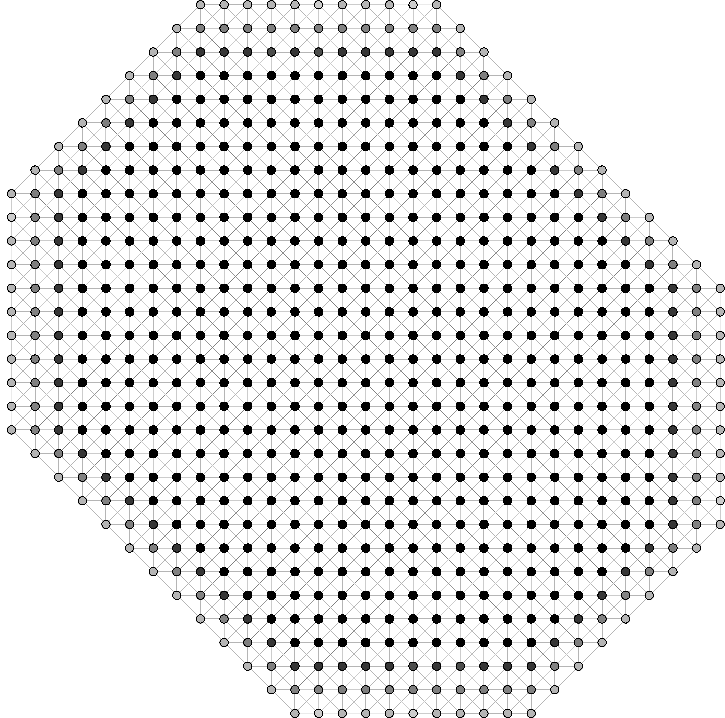
\includegraphics[height=8cm]{pictures/diagram.pdf}}
  \caption{The record illustrating maximal solution of the relaxed problem. This solution is obtained for the octagon $(10, 8, 10, 12, 10, 8, 10, 12)$. Since this is a relaxed problem (\ref{lp0})---(\ref{lp4}), the grayness in the Figure indicates the value of the move, that is a number between $0$ and $1$.  }
  \label{therecord}
  \end{figure}
%\todo{Do the record graph}

The record solution can be found in Figure \ref{therecord}. All \theoctagons relaxed problems were solved by {\tt gurobi} optimization software (see \cite{gurobi}) within 24 hours on a single core of a Linux machine equipped with {\tt Intel\textsuperscript{\textregistered}} {\tt Xeon\textsuperscript{\textregistered}} {\tt CPU X3220@2.40GHz} with 8GB of RAM.
\begin{proof}
  The proof is a calculation of $\obj_B$ for all octagons satisfying conditions (\ref{o1}) --- (\ref{o8}) of Lemma~\ref{lem:octagons}. The source code of the program {\tt generator.cpp} generating the relevant linear programs can be found in the repository~\cite{thewebpage}.
\end{proof}


\begin{corollary}
  The number of moves in a Morpion 5T game is bounded by $586$.
\end{corollary}

\section{MIP bound: \therecord}

\label{mip_bound}


%\begin{figure}[H]
\begin{wrapfigure}[10]{R}{0.55\textwidth}
\centering
\vspace{-50pt}
\begin{tikzpicture}[scale=0.6]
  \begin{semilogyaxis}[
    ymin=1,
    ymax=36033,
    log origin=infty,
    enlargelimits=false
  ]
    \addplot
      [const plot,fill=orange,draw=black]
      coordinates
        {(0,36033)    (2000,4644)  (4000,1302)   (6000,503)
         (8000,155) (10000,106)  (12000,71)  (14000,45)
         (16000,21) (18000,8)  (20000,1)}
  \closedcycle;
  \end{semilogyaxis}
\end{tikzpicture}
\caption{The vertical axis shows the number of cases and the horizontal axis shows the computation time in seconds. }
\label{histogram}
%\end{figure}
\end{wrapfigure}
Let us notice that results obtained in Theorem \ref{thm:linear_relax} can be naturally strengthened through longer computations. In practice, we were able to target 
%within two months of computations with three off--the--shelf Linux PC 
the objective 485. %\todo{Add more details about the machines and perhaps a graph with distribution of results (time). }


From Section \ref{linear_bound} we know all \theoctagons instances and their performance under relaxed (\ref{lp0})---(\ref{lp4}) linear problem. Apparently, out of all \theoctagons problems, \theinstances instances have the relaxed bound bigger or equal to 485. These are exactly the instances which must be treated by direct computations if we want to reduce the bound to 485. The total computation time for this target was approximately 310 days using the optimization software {\tt gurobi} (see \cite{gurobi}) on a single core of a Linux machine equipped with {\tt Intel\textsuperscript{\textregistered}} {\tt Xeon\textsuperscript{\textregistered}} {\tt CPU X3220@2.40GHz} with 8GB of RAM. The graph \ref{histogram} shows on the logarithmic scale the distribution of the computation time among \theinstances instances\footnote{In fact, a half of the instances required less than 100~sec. to reach the limit of \therecord and 9 instances required the computation time longer than 18000 seconds.}. 


% !TEX root = morpion5d.tex

\section{Geometry of Morpion Solitaire positions}
\label{sec:geometry}

%\todo{An introductory sentence}
In this section we collect a number of observations regarding geometric properties of Morpion Solitaire positions and formulate the basic definitions as well as the main result of this paper. 
In order to make linear computations feasible, we will limit the size of boards to rectangular ``boxes''.  In Section \ref{sec:gemmating} we explain why this is enough to solve the general problem of bounding the sequences in Morpion 5D. 
\begin{definition}
A box is a rectangular subset of ${\mathbb Z}^2$ bounded by $4$ edges parallel to the coordinate axes. A bounding box of a Morpion 5D position is the smallest box
containing this position. %rectangular part of the grid that contains this position
%edges parallel to the coordinate axes). 
\todo{Add a precise figure with a bounding box and dimensions, e.g. Figure~\ref{fig:small}}
\end{definition}

Every Morpion 5D graph contains the initial cross, hence the smallest bounding box has dimensions $9 \times 9$.
The graph depicted in Figure~\ref{fig:85} has a bounding box with dimensions $14 \times 13$.
However, the dimensions of the bounding box do not give information about the position of the initial cross inside. Since
this information is important for computations, we introduce the following %, which is important.
%We will employ the following convention.

\begin{notation*}
The distance of a bounding box to the initial cross can be described by $4$ numbers: the distances of the sides of the box to the edges of the cross. 
% is distances of its edges from the edges of the cross.
For graph depicted in Figure~\ref{fig:85} the distance from top edge of the cross to the top side of the bounding box is equal to $3$. For the right side it is $4$, for the bottom side it is $1$ and for the left side it is also $1$. 
The bounding box of the position in Figure~\ref{fig:85} is described as $(3,4,1,1)$.
\end{notation*}
  
\begin{table}[ht]
\centering
%
    \begin{tabular}{|l|l|l|l|}
    \hline
    No &  Bounding box &  Max size  \\
    \hline%
    
1&(3, 4, 1, 1)& 85.0\\
2&(3, 4, 2, 1)& 85.0\\
3&(4, 3, 1, 2)& 85.0\\
4&(4, 3, 1, 3)& 85.0\\
5&(2, 4, 2, 1)& 84.0\\
6&(2, 4, 2, 2)& 84.0\\
7&(2, 5, 1, 2)& 84.0\\
8&(2, 5, 2, 1)& 84.0\\
9&(2, 5, 2, 2)& 84.0\\
10&(3, 3, 1, 2)& 84.0\\
11&(3, 3, 2, 2)& 84.0\\
12&(3, 4, 1, 2)& 84.0\\
13&(3, 4, 1, 3)& 84.0\\
14&(3, 4, 2, 2)& 84.0\\
15&(3, 4, 3, 2)& 84.0\\
16&(4, 3, 0, 2)& 84.0\\
%
    \hline
    \end{tabular}%
\hspace*{5mm}
%
    \begin{tabular}{|l|l|l|l|}
    \hline
    No &  Bounding box &  Max size  \\
    \hline%
    
17&(4, 3, 2, 3)& 84.0\\
18&(2, 3, 2, 1)& 83.0\\
19&(2, 3, 2, 2)& 83.0\\
20&(2, 5, 1, 1)& 83.0\\
21&(3, 2, 1, 2)& 83.0\\
22&(3, 3, 1, 3)& 83.0\\
23&(3, 3, 3, 3)& 83.0\\
24&(3, 4, 2, 3)& 83.0\\
25&(3, 5, 1, 1)& 83.0\\
26&(3, 5, 2, 1)& 83.0\\
27&(4, 3, 0, 3)& 83.0\\
28&(4, 4, 0, 1)& 83.0\\
29&(4, 4, 0, 2)& 83.0\\
30&(4, 4, 1, 1)& 83.0\\
31&(4, 4, 1, 2)& 83.0\\
32&(4, 4, 1, 3)& 83.0\\
33&(4, 5, 1, 2)& 83.0\\
%
    \hline
    \end{tabular}%
 

\caption{Bounding boxes mentioned in Theorem \ref{thm:boxes}.\ref{thm:boxes:list} that admit Morpion 5D graphs of sizes $85$, $84$ and $83$. }
\label{tbl:boundingboxes}
\end{table}

Below we formulate the key theorem in this paper: %  \todo{Theorem, proved in Section 4, why is it important}
\begin{theorem}
\begin{enumerate}
\item Up to a symmetry every Morpion 5D {\em position} is contained in one of the following boxes:
$(4, 3, 3, 3)$, $(4, 4, 3, 2)$, $(5, 3, 2, 3)$, $(4, 3, 4, 2)$, $(5, 3, 3, 2)$, $(5, 4, 2, 1)$, 
$(6, 2, 2, 1)$, $(5, 4, 0, 2)$, $(5, 1, 4, 0)$. \label{thm:boxes:list}
\item Every box contained in one of the nine boxes listed in 1, with the exception of boxes $(6, 2, 2, 0)$ 
  and $(6, 0, 2, 0)$, is a bounding box of a Morpion 5D {\em graph}.
\item For each box $\mathcal{B}$ described in 2, the size of a maximal Morpion 5D graph with the bounding box $\mathcal{B}$ does not exceed $85$.
  Bounding boxes that admit Morpion 5D graphs of sizes greater than $82$ are listed 
    in Table~\ref{tbl:boundingboxes}. 
% All other boxes described in 2 are bounding boxes of graphs with size at most $82$.
\end{enumerate} 
\label{thm:boxes}
\end{theorem}
We will present a proof of this theorem in the next three sections with a summary of the argument in Subsection \ref{subsec:84}. 
In Section \ref{sec:linear} we precisely define the notion of a Morpion 5D graph. Intuitively, Morpion 5D graphs are obtained from Morpion 5D positions by forgetting about the order in which the moves were played.


%We will consider a class of graphs that are obtained from Morpion 5D positions by forgetting about 
%  the order in which the moves were played. %\todo{Definition of an unordered Morpion 5D graph}


%We will prove using linear programming that that the maximum size of  an unordered Morpion 5D graph with a bounding box equal to one of the bounding boxes listed in Table~\ref{tbl:boundingboxes}
% is $85$. \todo{This looks like a comment which should immediatelly after formulation of the theorem: it says, that we are not dealing
% with all morpion 5d graphs, but only with graphs generated by Morpion 5D positions - it is enough for the corollary that 85 is an upper bound -
% later there will be one more corollary improving on this bound to 84}

\begin{corollary}
\label{cor:84}
The longest sequence of moves in Morpion 5D does not exceed $84$.
\end{corollary}
\begin{proof} 
In Table \ref{tbl:boundingboxes} there are four bounding boxes with maximal graphs of size $85$. 
For these we formulate mixed integer problems with additional constraints that force the graph to
  be a Morpion 5D position.
These problems are much harder to solve, but with correct choice of solver optimization parameters we are able to show
  that there are no solutions of these problems of size $85$. Equipped with additional definitions and lemmas formulated later in this paper, in Subsection \ref{subsec:84} we add some technical 
information to this proof. 
\end{proof}


\printbibliography 
%\bibliographystyle{chicago}
%\bibliography{games.bib}


\end{document}